\documentclass[xcolor=dvipsnames]{beamer}

\usepackage{amsmath, amssymb, graphicx}
\usepackage[english]{babel}
\usepackage{times}
\usepackage[utf8]{inputenc}
\usepackage[T1]{fontenc}
\usepackage{listings}
\usepackage{hyperref}
\usepackage[norelsize,ruled,vlined]{algorithm2e}
\usepackage{color}
\usepackage{hyperref}
\usepackage{booktabs}
\usepackage{tikz}
\usetikzlibrary{arrows}
\usetikzlibrary{positioning}
\usetikzlibrary{shapes.multipart}

\newcommand{\fancyh}{\mathcal{H}}
\newcommand{\gangle}[1]{\langle{} #1 \rangle{}}
\newcommand{\myd}{\mathrm{d}}
\newcommand{\NN}{\mathbb{N}}
\newcommand{\ZZ}{\mathbb{Z}}

\mode<presentation>
{
    % \setbeamertemplate{navigation symbols}{}
    % \setbeamertemplate{items}[ball]
    % \setbeamertemplate{blocks}[rounded][shadow=true]
    \beamertemplatenavigationsymbolsempty
    \usecolortheme[named=Sepia]{structure}
    \usetheme{Malmoe}
    \useoutertheme{infolines}
    \setbeamercovered{transparent}
}

\lstset{language = [LaTeX]TeX,
    % captionpos=b,
    basicstyle= \small \ttfamily,
    keywordstyle = \bfseries \color{blue},
    commentstyle = \color{green}
}

\title[Monotone Data Flow Analysis Frameworks]{Monotone Data Flow Analysis Frameworks}
\author{Fengyun Liu, Ólafur Páll Geirsson}
\institute[EPFL]
{}
\date{\today}


% Delete this, if you do not want the table of contents to pop up at
% the beginning of each subsection:
\AtBeginSection[]
{\begin{frame}<beamer>{Overview}
        \tableofcontents[currentsection,
            currentsubsection,
            hideothersubsections,
            sectionstyle=show/shaded,
        subsectionstyle=show/shaded/hide]
    \end{frame}
}

\begin{document}

\tikzstyle{block} = [rectangle, draw, fill=blue!20, text centered, rounded corners, minimum height=1em]
\tikzstyle{line} = [draw, -latex']
\tikzstyle{value} = [rectangle, draw, fill=red!80, text centered, node distance=1.2cm]


%%%%%%%%%%%%%%%%%%%%%%%%%%%%%%%%%%%%%%%%%%%%%%%%%%%%%%%%%%%%%%%
% 0. Titlepage
%%%%%%%%%%%%%%%%%%%%%%%%%%%%%%%%%%%%%%%%%%%%%%%%%%%%%%%%%%%%%%%
\begin{frame}
    \titlepage{}
\end{frame}
\begin{frame}{Today's agenda}
    \tableofcontents[hideallsubsections]
\end{frame}

%%%%%%%%%%%%%%%%%%%%%%%%%%%%%%%%%%%%%%%%%%%%%%%%%%%%%%%%%%%%%%%
% 1. Background
%%%%%%%%%%%%%%%%%%%%%%%%%%%%%%%%%%%%%%%%%%%%%%%%%%%%%%%%%%%%%%%
\section{Background} % (fold)
\label{sec:Background}

\subsection{Flow graph}
\begin{frame}[fragile]{Triple $G = (N, E, n_0)$}
    \begin{center}
        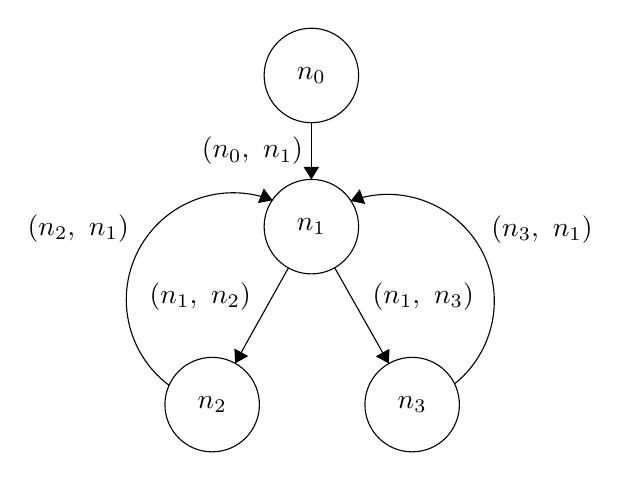
\begin{tikzpicture}[scale=0.2]
            \tikzstyle{every node}+=[inner sep=0pt]
            \draw [black] (24.7,-14) circle (3);
            \draw(24.7,-14) node {$n_0$};
            \draw [black] (24.7,-23.6) circle (3);
            \draw (24.7,-23.6) node {$n_1$};
            \draw [black] (18.4,-34.9) circle (3);
            \draw (18.4,-34.9) node {$n_2$};
            \draw [black] (31.1,-34.9) circle (3);
            \draw (31.1,-34.9) node {$n_3$};
            \draw [black] (15.682,-33.688) arc (-126.68179:-291.59948:6.793);
            \fill [black] (22.24,-21.93) -- (21.68,-21.17) -- (21.31,-22.1);
            \draw (13.14,-23.73) node [left] {$(n_2,\mbox{ }n_1)$};
            \draw [black] (27.192,-21.975) arc (110.40413:-51.35216:6.765);
            \fill [black] (27.19,-21.97) -- (28.12,-22.16) -- (27.77,-21.23);
            \draw (36.1,-23.76) node [right] {$(n_3,\mbox{ }n_1)$};
            \draw [black] (23.24,-26.22) -- (19.86,-32.28);
            \fill [black] (19.86,-32.28) -- (20.69,-31.82) -- (19.81,-31.34);
            \draw (20.89,-28.05) node [left] {$(n_1,\mbox{ }n_2)$};
            \draw [black] (26.18,-26.21) -- (29.62,-32.29);
            \fill [black] (29.62,-32.29) -- (29.66,-31.35) -- (28.79,-31.84);
            \draw (28.56,-28.03) node [right] {$(n_1,\mbox{ }n_3)$};
            \draw [black] (24.7,-17) -- (24.7,-20.6);
            \fill [black] (24.7,-20.6) -- (25.2,-19.8) -- (24.2,-19.8);
            \draw (24.2,-18.8) node [left] {$(n_0,\mbox{ }n_1)$};
        \end{tikzpicture}
    \end{center}
\end{frame}
\subsection{Semilattice}
\begin{frame}[fragile]{Set $L$ with \emph{meet} operation $\wedge$}
    \begin{align*}
        a \wedge a & = a & (idempotent) \\
        a \wedge b & = b \wedge a & (commutative) \\
        a \wedge (b \wedge c) & = (a \wedge b) \wedge c & (associative)
    \end{align*}
\end{frame}
\subsection{Semilattice: ordering}
\begin{frame}[fragile]{$\wedge$ defines an order on $L$}
    \begin{align*}
        a & \leqq b & \text{iff } a \wedge b = b \\
        a < b & = b \wedge a & \text{iff } a \wedge b = b \text{\ and } a \neq b
    \end{align*}
\end{frame}
\subsection{Semilattice: 0 and 1}
\begin{frame}[fragile]{}
    \begin{block}{Zero element (bottom?): 0}
        Element $e \in L$ is called zero, labeled 0, if
        \[
            e \wedge x = e \qquad \forall x \in L
        \]
    \end{block}
    \begin{block}{One element (top?): 1}
        Element $e \in L$ is called one, labeled 1, if
        \[
            e \wedge x = x \qquad \forall x \in L
        \]
    \end{block}
\end{frame}
\subsection{Semilattice: bounded chains}
\begin{frame}[fragile]{} % {Chain $x_1, x_2, \ldots, x_n$}
    \begin{block}{Chain}
        A sequence $x_1, x_2, \ldots, x_n$ forms a \emph{chain} if $x_i > x_{i + 1}$ for $1 \leqq i < n$.
    \end{block}
    \begin{block}{Bounded chain}
        A chain is said to be \emph{bounded} if for each $x \in L$ there is a constant $b_x$ such that each chain beginning with $x$ has length at most $b_x$.
    \end{block}
\end{frame}

%%%%%%%%%%%%%%%%%%%%%%%%%%%%%%%%%%%%%%%%%%%%%%%%%%%%%%%%%%%%%%%
% 2. Monotone Data Flow Analysis Frameworks
%%%%%%%%%%%%%%%%%%%%%%%%%%%%%%%%%%%%%%%%%%%%%%%%%%%%%%%%%%%%%%%
\section{Monotone Data Flow Analysis Frameworks} % (fold)
\label{sec:mdfaf}

% section Monotone Data Flow Analysis Frameworks (end)
%%%%%%%%%%%%%%%%%%%%%%%%%%%%%%%%%%%%%%%%%%%%%%%%%%%%%%%%%%%%%%%
% 3. Approaches to solving Monotone Data Flow Analysis Frameworks
%%%%%%%%%%%%%%%%%%%%%%%%%%%%%%%%%%%%%%%%%%%%%%%%%%%%%%%%%%%%%%%
\section{Approaches to solving MDFAF} % (fold)
\label{sec:approaches}

% section approaches
%%%%%%%%%%%%%%%%%%%%%%%%%%%%%%%%%%%%%%%%%%%%%%%%%%%%%%%%%%%%%%%
% 4. A Variant of Kildall's Algorithm
%%%%%%%%%%%%%%%%%%%%%%%%%%%%%%%%%%%%%%%%%%%%%%%%%%%%%%%%%%%%%%%
\section{A Variant of Kildall's Algorithm} % (fold)
\label{sec:variant}

% section A Variant of Kildall's Algorithm


\subsection{The Algorithm}

\begin{frame}
  \frametitle{Initialization}

  \begin{columns}[onlytextwidth]
    \begin{column}{0.5\textwidth}
      \begin{equation*}
        B[n] =
        \begin{cases}
          f_{n_0}(0) & \text{if } n = n_0\\
          1 & otherwise
        \end{cases}
      \end{equation*}

      \begin{itemize}
      % \item \textit{Initialization}
      \item 0 - zero element of the lattice
      \item 1 - one element of the lattice
      \item $f_{n_0}$ - the function that $n_0$ corresponds to
      \end{itemize}
    \end{column}

    \begin{column}{0.5\textwidth}
        \begin{center}
            \begin{tikzpicture}[node distance = 2cm, auto, every text node part/.style={align=left}]
                % Place nodes
                \node [block, label=above:$n_0$] (n0) {$A = 1$};
                \node [value, right of=n0, node distance=1.1cm] (s0) {\tiny \{A=1\}};
                \node [block, below left of=n0, label=above:$n_1$] (n1) {$A = 2$\\$B = 3$};
                \node [value, left of=n1, node distance=0.9cm] (s1) {\tiny 1};
                \node [block, below right of=n0, label=above:$n_2$] (n2) {$A = 3$\\$B = 2$};
                \node [value, right of=n2, node distance=0.9cm] (s2) {\tiny 1};
                \node [block, below right of=n1, label=above:$n_3$] (n3) {$C = A + B$};
                \node [value, right of=n3, node distance=1.3cm] (s3) {\tiny 1};
                % Draw edges
                \path [line] (n0) -- (n1);
                \path [line] (n0) -- (n2);
                \path [line] (n1) -- (n3);
                \path [line] (n2) -- (n3);
            \end{tikzpicture}
        \end{center}
    \end{column}

  \end{columns}
\end{frame}

\subsection{Step 2}

\begin{frame}
  \frametitle{A Variant of Kildall's Algorithm - Iteration Step}
  \begin{columns}
    \begin{column}
      \begin{itemize}
      \item \textit{Iteration Step}. Visit nodes other than $n_0$ in order $n_1, n_2, ...$, (not fixed in advance and with repetitions). We visit node $n$ by setting \\
        \begin{equation*}
          B[n] = \bigwedge_{p \in PRED(n)} f_n(B[p])
        \end{equation*}
      \end{itemize}
    \end{column}

    \begin{column}
      \begin{tikzpicture}[node distance = 2cm, auto, every text node part/.style={align=left}]
          % Place nodes
        \node [block, label=above:$n_0$] (n0) {$A = 1$};
        \node [value, right of=n0, node distance=1.1cm] (s0) {\tiny \{A=1\}};
        \node [block, below left of=n0, label=above:$n_1$] (n1) {$A = 2$\\$B = 3$};
        \node [value, above of=n1, node distance=0.8cm, xshift=-0.4cm] (s1) {\tiny 1};
        \node [block, below right of=n0, label=above:$n_2$] (n2) {$A = 3$\\$B = 2$};
        \node [value, left of=n2, node distance=0.9cm] (s2) {\tiny 1};
        \node [block, below right of=n1, label=above:$n_3$] (n3) {$C = A + B$};
        \node [value, right of=n3, node distance=1.3cm] (s3) {\tiny 1};
        % Draw edges
        \path [line] (n0) -- (n1);
        \path [line] (n0) -- (n2);
        \path [line] (n1) -- (n3);
        \path [line] (n2) -- (n3);
      \end{tikzpicture}
    \end{column}
  \end{columns}
\end{frame}

\subsection{Step 3}

\begin{frame}
  \frametitle{A Variant of Kildall's Algorithm - Final Step}
  \begin{itemize}
  \item \textit{Final Step}. Set \\
    \begin{equation*}
      H[n] =
      \begin{cases}
        0 & \text{if } n = n_0\\
        \bigwedge_{p \in PRED(n)} B[p] & otherwise
      \end{cases}
    \end{equation*}
  \end{itemize}
\end{frame}

%%%%%%%%%%%%%%%%%%%%%%%%%%%%%%%%%%%%%%%%%%%%%%%%%%%%%%%%%%%%%%%
% 5. Undecidability
%%%%%%%%%%%%%%%%%%%%%%%%%%%%%%%%%%%%%%%%%%%%%%%%%%%%%%%%%%%%%%%
\section{Undecidability of MOP Problem for MDFAF} % (fold)
\label{sec:undecidability}

% section undecidability (end)
\begin{frame}[fragile]{Example usage of blocks and columns}
    \begin{columns}
        \begin{column}{0.5\textwidth}
            \begin{block}{Block 1}
                \begin{itemize}
                    \item<1> 1
                    \item<2> 2
                    \item<3> 3
                \end{itemize}
            \end{block}
        \end{column}
        \begin{column}{0.5\textwidth}
            \begin{block}{Block 2}
                \begin{itemize}
                    \item<4> b
                    \item<5> b
                    \item<6> b
                \end{itemize}
            \end{block}
        \end{column}
    \end{columns}
\end{frame}
\end{document}
